\section{Introduction}\label{sec:intro}

Multimodal foundation models such as CLIP~\cite{radford2021clip} and
ImageBind~\cite{girdhar2023imagebind} map heterogeneous signals (images,
text, audio) into a shared vector space for cross-modal vector similarity
search~\cite{jia2021align}. At deployment scale, storage becomes the
bottleneck: high-dimensional \texttt{float32} embeddings can require terabytes of RAM,
motivating approximate nearest neighbor (ANN) indexes that compress to a few bytes per
vector~\cite{jegou2011pq,gao2024rabitq}.\looseness=-1

Binary quantization (BQ) is the extreme compression point:
RaBitQ~\cite{gao2024rabitq} reaches $32\times$ compression by encoding each
dimension as one sign bit relative to the dataset centroid. Its production
adoption in Apache Lucene BBQ and extension to multi-bit
Extended-RaBitQ~\cite{gao2025extended} show BQ indexing is now
practically deployed.\looseness=-1

\begin{figure}[!t]
  \centering
  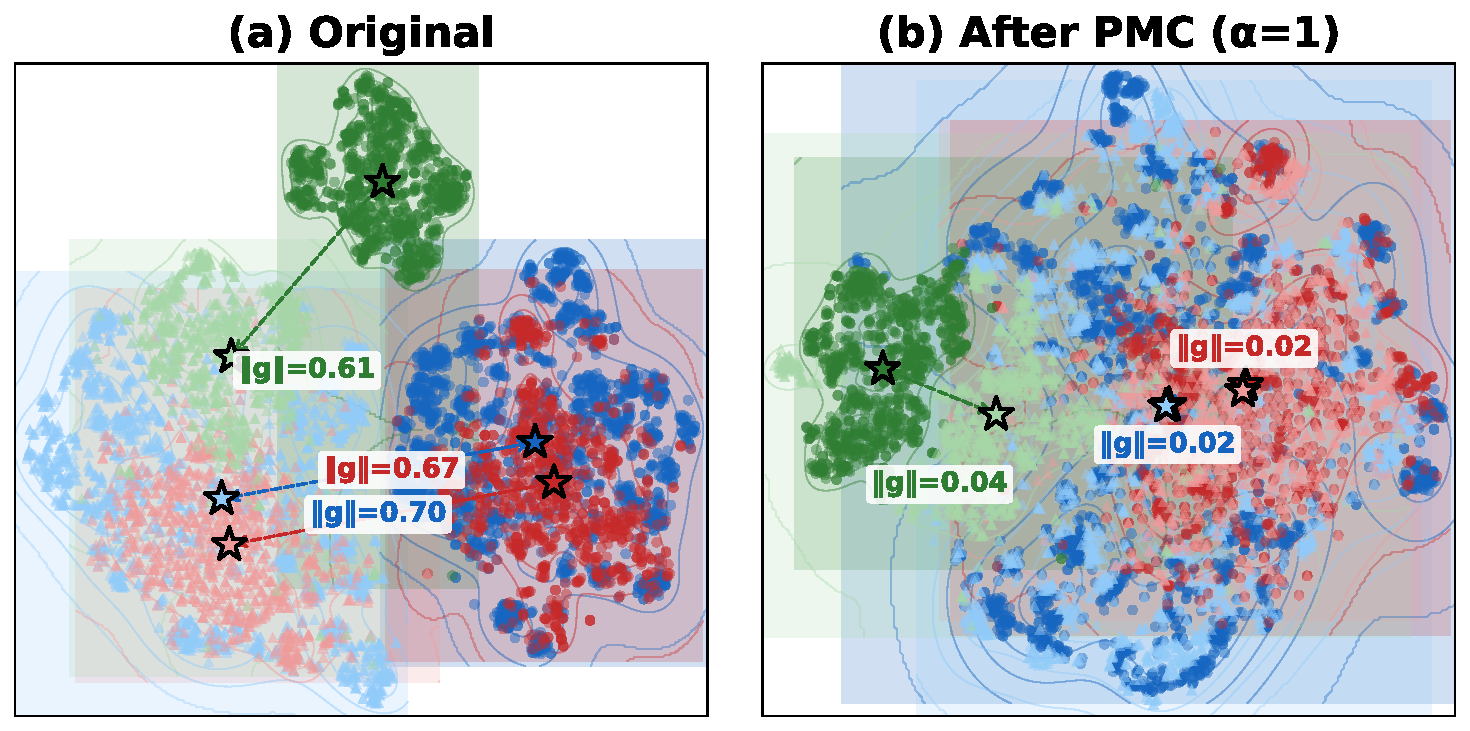
\includegraphics[width=\columnwidth]{figures/fig1_tsne.pdf}
  \Description{t-SNE visualization of ImageBind embeddings from three cross-modal datasets (MSCOCO, Flickr30K, Clotho) before and after PMC correction. Panel (a) shows separated modality clusters in the original space; panel (b) shows aligned clusters after PMC at alpha equals one.}
  \caption{t-SNE of ImageBind embeddings. (a)~Each modality forms a separate cluster. (b)~After PMC ($\alpha{=}1$), paired modalities overlap. Blue\,=\,MSCOCO, red\,=\,Flickr30K, green\,=\,Clotho; dark\,=\,DB, light\,=\,query.}\label{fig:modality-gap}
\end{figure}

{\emergencystretch=1em
These methods rely on a shared-centroid residual premise: queries and database
vectors are drawn from the same distribution and share a common centroid. Cross-modal
retrieval violates this assumption---\hspace{0pt}queries from one modality cluster around
a different centroid than the database vectors.\looseness=-1\par}

This \emph{modality gap}~\cite{liang2022mind} is particularly harmful to BQ
because the encoding $\mathrm{sign}(x_i - c_i)$ has \emph{zero
error margin}: the decision boundary passes exactly through the centroid,
and any systematic displacement causes structured bit corruption that
scales with gap magnitude (Figure~\ref{fig:modality-gap}); an oracle test confirms this: same-modality queries ($\|\mathbf{g}\|{=}0$) reach R@100$=$0.84 under RaBitQ, versus 0.57 for cross-modal queries ($\|\mathbf{g}\|{=}0.82$).
Prior work addresses cross-modal retrieval through graph
augmentation~\cite{chen2024roargraph,jaiswal2022ood}, encoder
fine-tuning~\cite{eslami2025alignclip}, or embedding-space
calibration~\cite{li2025grclip}, but none targets compressed ANN indexes
where centroid misalignment corrupts both Inverted File (IVF) routing and binary
codes.\looseness=-1

In this paper, we first analyze how the modality gap degrades BQ ANN indexes at two coupled stages---IVF routing and binary
code formation---and show that dimensions with concentrated gap energy
are most vulnerable to boundary crossing; a selective correction test
confirms that correcting only the highest-gap dimensions recovers most
of the gain.
Based on this analysis, we propose Per-Modality Centroid Correction
(PMC), a one-time build-time alignment that shifts database vectors
toward the query centroid before index construction. Unlike query-only
mean shift, which leaves IVF centroids and quantized codes misaligned,
PMC exploits the centroid's dual role as IVF routing pivot and sign-bit decision boundary, rewriting both at the source with no serving-time query transform and no additional index memory
(Figure~\ref{fig:pmc-overview}). We validate PMC across five cross-modal benchmarks including 407M-scale LAION, three multimodal encoders, and four BQ index types. Our contributions:
\begin{itemize}[nosep,leftmargin=*,topsep=0pt]
\item We show that the modality gap corrupts both IVF routing and binary codes, with recall loss scaling with gap magnitude.
\item We discover that this corruption concentrates in a few high-$|g_i|$ dimensions; a selective PMC variant correcting only those recovers most recall.
\item We propose PMC, a zero-cost build-time correction ($\alpha{=}1$) that realigns routing and codes via the centroid's dual role; ablation confirms DB-side over query-side correction.
\end{itemize}

\begin{figure}[t]
  \centering
  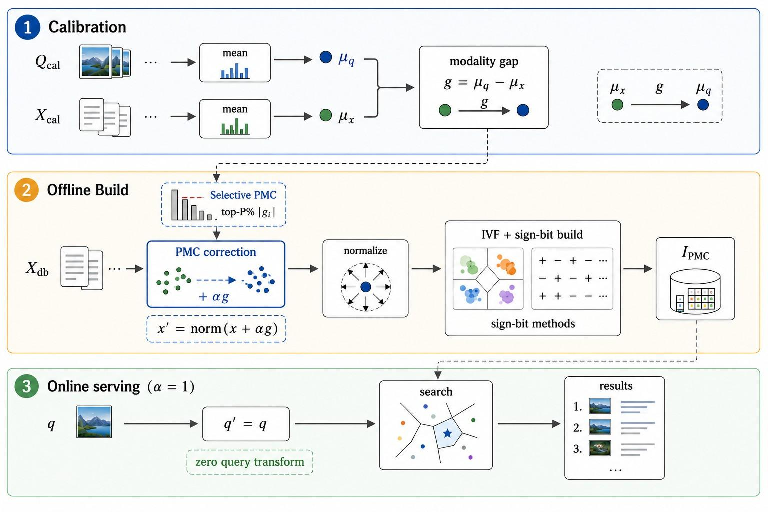
\includegraphics[width=\columnwidth]{figures/fig2_overview.pdf}
  \caption{PMC workflow: calibration estimates $\boldsymbol{\mu}_q$, $\boldsymbol{\mu}_x$, and $\mathbf{g}{=}\boldsymbol{\mu}_q-\boldsymbol{\mu}_x$; offline build shifts/normalizes database vectors before BQ index construction; at $\alpha{=}1$, online serving uses $\mathbf{q}'{=}\mathbf{q}$ and searches $\mathcal{I}_{\mathrm{PMC}}$.}
  \Description{Three-lane landscape PMC overview. Lane 1 (Calibration / Gap Estimation) takes calibration query and database samples, computes means mu-q and mu-x, and outputs the modality gap g equals mu-q minus mu-x, with an inset showing the centroid shift from mu-x to mu-q. Lane 2 (Offline Build / PMC Index Construction) takes database vectors, includes an optional selective PMC box that keeps only top-P dimensions of g, applies PMC correction x plus alpha g and normalization x-prime equals norm(x plus alpha g), then performs IVF-based BQ index build listing BinaryFlat, BinaryIVF, BBQ, and RaBitQ to produce I-PMC. Lane 3 (Online Serving / Search, alpha equals 1) shows no query transform q-prime equals q, then search over I-PMC and ranked results; dashed arrows indicate dependency from g to offline correction and from I-PMC to search.}
  \label{fig:pmc-overview}
\end{figure}
